% Provenance (never printed): see sources/outline_sources.md (Year 3:
% concordia and discordia; 40Ar/39Ar step heating; Sm-Nd model ages;
% cosmogenic nuclides; fission tracks and (U-Th)/He). Brief:
% sources/book5/BRIEFS.md, ch. 13. Curves from figdata/bachelor-3/
% concordia.py, arar_spectrum.py, model_ages.py, cosmogenic.py. Exercise and
% problem values in the Book 5 scratch calculator calc/ch13.py. The zircons,
% the biotite spectrum, the Nd sample and the helium ages of the Varden
% granite are invented, consistent with the Year 1 volume's granite of 310 Ma.
\chapter{Geocronologia avançada}\label{ch:b3:advanced-geochronology}

Um cristal de zircão de um décimo de milímetro de comprimento mantém dois relógios em funcionamento
desde que seu granito cristalizou: urânio-238 decaindo para chumbo-206 e
urânio-235 decaindo para chumbo-207. Quando os dois relógios concordam, a idade
está além de dúvida. Quando discordam, a própria discordância pode ser datada: o
cristal perdeu parte de seu chumbo em um evento posterior, e os dois relógios, lidos
em conjunto, fornecem a idade do granito e a idade do evento. Este capítulo
lê vários relógios ao mesmo tempo, em urânio e chumbo, em argônio, em neodímio, em
traços de fissão e hélio, e em átomos raros produzidos por raios cósmicos, e diz
até onde cada idade pode ser confiável.

\begin{recall}
O decaimento radioativo, a equação da idade, a isócrona e sua razão inicial, a
reta de mínimos quadrados, decaimento ramificado, idade potássio--argônio, temperatura de
fechamento e idade de resfriamento estão no volume do primeiro ano, em seu capítulo sobre
datação radiométrica; a fórmula de erosão em regime estacionário dos \omterm{def:b3:advanced-geochronology:cosmogenic}{nuclídeos cosmogênicos} está em
seu capítulo sobre erosão e transporte. O reservatório uniforme condrítico, a
notação épsilon e o manto empobrecido estão no volume do segundo ano, em seu
capítulo sobre geoquímica isotópica; ionização térmica e espectrometria de massa
multicoletora em seu capítulo sobre métodos de campo e de laboratório. \omterm{def:b3:orogenic-wedges:thermochronology}{Termocronologia} e
a \omterm{def:b3:orogenic-wedges:age-elevation}{relação idade--altitude} estão no \cref{ch:b3:orogenic-wedges}.
\end{recall}

\section{Urânio, chumbo e a concórdia}\label{sec:b3:advanced-geochronology:upb}

O urânio tem dois isótopos de vida longa. O urânio-238 decai por uma cadeia de
filhas de vida curta até o chumbo-206, com $\lambda_{238} =
\qty{1.55125e-10}{yr^{-1}}$; o urânio-235 decai para chumbo-207 com $\lambda_{235}
= \qty{9.8485e-10}{yr^{-1}}$, seis vezes mais rápido. Sua razão atual é
$^{235}\mathrm{U}/^{238}\mathrm{U} = 0.0072567$, ou $^{238}\mathrm{U}/^{235}\mathrm{U}
= 137.8$, a mesma em toda rocha terrestre. O zircão, $\mathrm{ZrSiO_4}$, incorpora
muito urânio e quase nenhum chumbo ao crescer, e resiste ao intemperismo
e sobrevive ao metamorfismo: quase todo o seu chumbo é radiogênico.
% ledger: amherst:constants, tulane:upb-zircon

Sejam $x = {}^{207}\mathrm{Pb}^*/{}^{235}\mathrm{U}$ e $y =
{}^{206}\mathrm{Pb}^*/{}^{238}\mathrm{U}$ as razões atuais do chumbo radiogênico
em relação ao seu isótopo-pai. Cada uma fornece uma idade, $t_{206} = \ln(1 + y)/\lambda_{238}$
e $t_{207} = \ln(1 + x)/\lambda_{235}$.

\begin{definition}[Concórdia, discórdia, interceptos, diagrama de Tera--Wasserburg]
\label{def:b3:advanced-geochronology:concordia}
A \emph{concórdia}\index{concórdia} é a curva do plano $(x, y)$ sobre o qual
as duas idades urânio--chumbo são iguais. Uma \emph{discórdia}\index{discórdia}
é uma reta ao longo da qual se alinham análises discordantes de uma população de
cristais; suas interseções com a concórdia são o
\emph{intercepto superior}\index{intercepto superior} (o mais antigo) e o
\emph{intercepto inferior}\index{intercepto inferior} (o mais jovem). O
\emph{diagrama de Tera--Wasserburg}\index{diagrama de Tera--Wasserburg} representa
$X = {}^{238}\mathrm{U}/{}^{206}\mathrm{Pb}^*$ contra $Y =
{}^{207}\mathrm{Pb}^*/{}^{206}\mathrm{Pb}^*$.
\end{definition}

\begin{theorem}[A concórdia]\label{thm:b3:advanced-geochronology:concordia}
Um cristal que permaneceu fechado ao urânio e ao chumbo desde sua formação, há um
tempo $t$, situa-se em
\[
C(t) = \bigl(e^{\lambda_{235}t} - 1,\; e^{\lambda_{238}t} - 1\bigr).
\]
À medida que $t$ cresce, a curva sobe cada vez mais devagar em relação a $x$: sua inclinação,
$\mathrm dy/\mathrm dx = (\lambda_{238}/\lambda_{235})\,e^{(\lambda_{238} -
\lambda_{235})t}$, decresce a partir de $\lambda_{238}/\lambda_{235} = 0.1575$ na
origem, de modo que a \omterm{def:b3:advanced-geochronology:concordia}{concórdia} é côncava voltada para o eixo $x$.
\end{theorem}

\begin{proof}
Para cada isótopo-pai, o número de filhas radiogênicas por átomo-pai restante é
$e^{\lambda t} - 1$, a equação da idade do volume do primeiro ano. Derivando
ambas as coordenadas em relação a $t$ e dividindo-as obtém-se a inclinação; como
$\lambda_{235} > \lambda_{238}$, ela decresce com $t$.
\end{proof}

O chumbo é um íon grande que se acomoda mal na rede do zircão. Nas partes de um
cristal danificadas pela própria radioatividade, ele pode escapar em um evento posterior de
aquecimento ou circulação de fluidos.
% ledger: tulane:upb-zircon

\begin{theorem}[A perda episódica de chumbo gera uma corda]\label{thm:b3:advanced-geochronology:discordia}
Um cristal formado há um tempo $t_1$ que perdeu, há um tempo $t_2$, uma fração $f$
de seu chumbo radiogênico, e permaneceu fechado no resto, situa-se hoje em
\[
(1 - f)\,C(t_1) + f\,C(t_2),
\]
sobre a corda que une os pontos $t_1$ e $t_2$ da \omterm{def:b3:advanced-geochronology:concordia}{concórdia}. Cristais que
perderam frações diferentes situam-se ao longo dessa corda, uma \omterm{def:b3:advanced-geochronology:concordia}{discórdia} cujo \omterm{def:b3:advanced-geochronology:concordia}{intercepto superior}
é $t_1$ e cujo \omterm{def:b3:advanced-geochronology:concordia}{intercepto inferior} é $t_2$.
\end{theorem}

\begin{proof}
Considera-se um sistema de decaimento, de constante $\lambda$, e conta-se por átomo-pai
presente hoje. Há um tempo $t_2$ existiam $e^{\lambda t_2}$ átomos-pai, e
filhas radiogênicas $e^{\lambda t_2}(e^{\lambda(t_1 - t_2)} - 1) =
e^{\lambda t_1} - e^{\lambda t_2}$. O evento deixou $(1 - f)(e^{\lambda t_1} -
e^{\lambda t_2})$; desde então o pai produziu mais $e^{\lambda t_2} - 1$. A
soma é $(1 - f)(e^{\lambda t_1} - 1) + f(e^{\lambda t_2} - 1)$. Os dois isótopos
de chumbo se comportam quimicamente do mesmo modo, logo $f$ é o mesmo para ambos, e as duas
coordenadas se combinam no ponto enunciado.
\end{proof}

\begin{omfigure}
\begin{tikzpicture}
\begin{groupplot}[group style={group size=2 by 1, horizontal sep=1.7cm},
  omrecord, width=0.47\linewidth, height=0.42\linewidth, title style={font=\small},
  tick label style={font=\scriptsize}, label style={font=\small}]
\nextgroupplot[title={(a) diagrama da concórdia},
  xlabel={$^{207}\mathrm{Pb}^*/^{235}\mathrm{U}$}, ylabel={$^{206}\mathrm{Pb}^*/^{238}\mathrm{U}$},
  xmin=0.04, xmax=0.44, ymin=0.006, ymax=0.06,
  xtick={0.1,0.2,0.3,0.4}, xticklabels={0.1,0.2,0.3,0.4},
  ytick={0.01,0.02,0.03,0.04,0.05}, yticklabels={0.01,0.02,0.03,0.04,0.05},
  scaled ticks=false]
% computed in figdata/bachelor-3/concordia.py
\addplot[black, thick] table[x=xw, y=yw] {figdata/out/bachelor-3-concordia-curve.dat};
\addplot[black, only marks, mark=*, mark size=1.4pt, nodes near coords={\scriptsize\pgfmathprintnumber[fixed, precision=0]{\pgfplotspointmeta}},
  point meta=explicit, nodes near coords align={anchor=south east},
  restrict expr to domain={\thisrow{t}}{100:350}]
  table[x=xw, y=yw, meta=t] {figdata/out/bachelor-3-concordia-ticks.dat};
\addplot[omDef, thick, densely dashed] table[x=x, y=y] {figdata/out/bachelor-3-concordia-line.dat};
\addplot[red!70!black, only marks, mark=diamond*, mark size=2pt] table[x=x, y=y] {figdata/out/bachelor-3-concordia-zircons.dat};
\nextgroupplot[title={(b) diagrama de Tera--Wasserburg},
  xlabel={$^{238}\mathrm{U}/^{206}\mathrm{Pb}^*$}, ylabel={$^{207}\mathrm{Pb}^*/^{206}\mathrm{Pb}^*$},
  xmin=15, xmax=75, ymin=0.0465, ymax=0.0535,
  ytick={0.047,0.049,0.051,0.053}, yticklabels={0.047,0.049,0.051,0.053},
  scaled ticks=false]
\addplot[black, thick] table[x=xtw, y=ytw] {figdata/out/bachelor-3-concordia-curve.dat};
\addplot[black, only marks, mark=*, mark size=1.4pt, nodes near coords={\scriptsize\pgfmathprintnumber[fixed, precision=0]{\pgfplotspointmeta}},
  point meta=explicit, nodes near coords align={anchor=north east},
  restrict expr to domain={\thisrow{t}}{100:250}]
  table[x=xtw, y=ytw, meta=t] {figdata/out/bachelor-3-concordia-ticks.dat};
\addplot[omDef, thick, densely dashed] table[x=xtw, y=ytw] {figdata/out/bachelor-3-concordia-twline.dat};
\addplot[red!70!black, only marks, mark=diamond*, mark size=2pt] table[x=xtw, y=ytw] {figdata/out/bachelor-3-concordia-zircons.dat};
\end{groupplot}
\end{tikzpicture}

\par\smallskip{\small (a) A \omterm{def:b3:advanced-geochronology:concordia}{concórdia}, com suas idades em milhões de anos,
e cinco zircões discordantes inventados de um granito (em vermelho; suas elipses de erro
são menores que os símbolos), alinhados sobre uma \omterm{def:b3:advanced-geochronology:concordia}{discórdia} (tracejada) que
encontra a \omterm{def:b3:advanced-geochronology:concordia}{concórdia} perto de 311 e \qty{100}{\Ma}. (b) Os mesmos zircões e a mesma reta
no \omterm{def:b3:advanced-geochronology:concordia}{diagrama de Tera--Wasserburg}, em que uma \omterm{def:b3:advanced-geochronology:concordia}{discórdia} continua sendo uma
reta.}\label{fig:b3:advanced-geochronology:concordia}
\end{omfigure}
% ledger: amherst:constants

Os interceptos são encontrados onde $a + b\,x(t) = y(t)$, uma equação em $t$ que é
resolvida pelo método de Newton: com $g(t) = e^{\lambda_{238}t} - 1 - a -
b(e^{\lambda_{235}t} - 1)$ e $g'(t) = \lambda_{238}e^{\lambda_{238}t} -
b\lambda_{235}e^{\lambda_{235}t}$, itera-se $t \leftarrow t - g/g'$ a partir de uma estimativa
próxima de cada intercepto. Três propriedades do resultado são importantes na prática.
Primeiro, o \omterm{def:b3:advanced-geochronology:concordia}{intercepto superior} só é preciso se a \omterm{def:b3:advanced-geochronology:concordia}{discórdia} cruza a \omterm{def:b3:advanced-geochronology:concordia}{concórdia} em um ângulo
grande. Uma \omterm{def:b3:advanced-geochronology:concordia}{discórdia} jovem, como na figura acima, corre quase ao longo da \omterm{def:b3:advanced-geochronology:concordia}{concórdia},
e uma pequena mudança em sua inclinação desloca o
intercepto para muito longe. Segundo, se a perda de chumbo é recente, $t_2 = 0$, a \omterm{def:b3:advanced-geochronology:concordia}{discórdia}
passa pela origem, e todo cristal tem a mesma
razão $^{207}\mathrm{Pb}^*/^{206}\mathrm{Pb}^*$,
\[
\frac{^{207}\mathrm{Pb}^*}{^{206}\mathrm{Pb}^*} = \frac{1}{137.8}\,
\frac{e^{\lambda_{235}t_1} - 1}{e^{\lambda_{238}t_1} - 1},
\]
que fornece $t_1$ sem o urânio: a idade chumbo--chumbo. Terceiro, uma reta no
diagrama da \omterm{def:b3:advanced-geochronology:concordia}{concórdia}, $x = (y - a)/b$, torna-se nas
coordenadas de Tera--Wasserburg $Y = (1 - aX)/(137.8\,b)$, novamente uma reta. O
\omterm{def:b3:advanced-geochronology:concordia}{diagrama de Tera--Wasserburg} usa razões medidas diretamente, sem necessidade de calcular o urânio-235
a partir do urânio-238, e uma mistura com chumbo comum, não radiogênico e rico em
chumbo-207, plota-se em uma reta que atinge o eixo $Y$ na razão do chumbo
comum.

As idades urânio--chumbo são medidas de duas maneiras. Cristais isolados ou fragmentos,
dissolvidos depois de as zonas danificadas terem sido removidas por dissolução parcial
e de seu chumbo e urânio terem sido separados, são medidos por espectrometria de massa
por ionização térmica, com as idades mais precisas da geologia. Pontos de algumas dezenas de
micrômetros de diâmetro são medidos no lugar, por sonda iônica ou por ablação a laser,
com menor precisão, mas zona por zona através de um cristal que cresceu em
vários eventos.

\begin{inthelab}[O laboratório de geocronologia]
\begin{minipage}[t]{0.55\linewidth}\vspace{0pt}
A datação de um zircão começa com uma rocha triturada e termina em um laboratório limpo. Os
geocronologistas separam os zircões por densidade e magnetismo, escolhem os
cristais mais límpidos sob o microscópio binocular e fazem imagens de seu zoneamento. Os
cristais são parcialmente dissolvidos para remover suas zonas danificadas e, em seguida, dissolvidos
por completo com um traçador isotópico de composição conhecida, e o urânio e o chumbo são
separados em pequenas colunas de resina, em ar filtrado para afastar o chumbo da
poeira. Um espectrômetro de massa mede as razões isotópicas. As amostras de argônio seguem um
caminho diferente: um reator, depois uma linha de gás em que um laser aquece cada etapa e
o argônio é purificado antes do espectrômetro.
\end{minipage}\hfill
\begin{minipage}[t]{0.42\linewidth}\vspace{0pt}
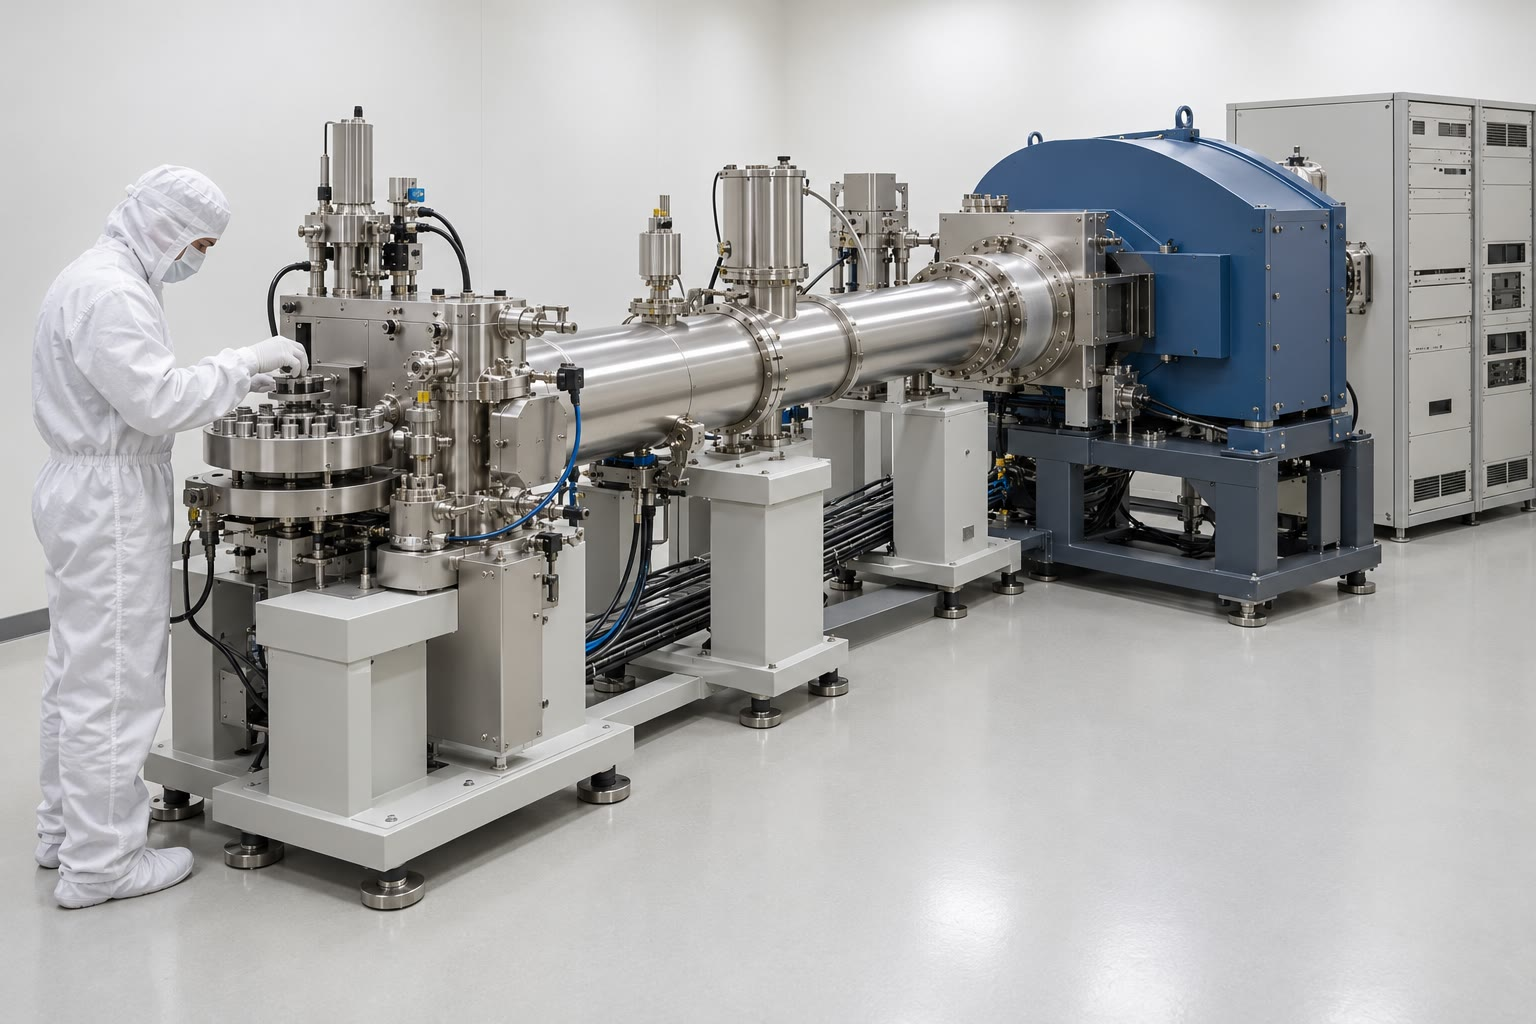
\includegraphics[width=\linewidth]{images/book5/ai/b3-mass-spec-lab.jpg}

{\scriptsize Um espectrômetro de massa em laboratório limpo: a torre de amostras à
esquerda, o tubo de voo e o eletroímã (Ilustração gerada
por IA.)}
\end{minipage}
\end{inthelab}

\section{Datação argônio--argônio}\label{sec:b3:advanced-geochronology:arar}

O método potássio--argônio do volume do primeiro ano mede o potássio e
o argônio em duas alíquotas separadas de um mineral. O método argônio--argônio
mede apenas argônio, em uma alíquota, como razões de isótopos. A amostra é
irradiada com nêutrons rápidos no núcleo de um reator nuclear, onde a
reação $^{39}\mathrm{K}(n,p)^{39}\mathrm{Ar}$ transforma uma fração fixa do seu
potássio-39 em argônio-39, um indicador do potássio. Um mineral de idade conhecida, o
monitor, é irradiado ao lado dela.
% ledger: nmgrl:arar, amherst:arar

\begin{definition}[Datação argônio--argônio, fator J, espectro de idades, idade de platô]
\label{def:b3:advanced-geochronology:arar}
A \emph{datação $^{40}\mathrm{Ar}/^{39}\mathrm{Ar}$}\index{datação argônio--argônio@$^{40}\mathrm{Ar}/^{39}\mathrm{Ar}$ datação}
data um mineral portador de potássio pela razão $R =
{}^{40}\mathrm{Ar}^*/{}^{39}\mathrm{Ar}_{\mathrm K}$ de seu argônio-40
radiogênico para o argônio-39 produzido a partir de seu potássio por irradiação com nêutrons. O
\emph{fator J}\index{fator J} de uma irradiação é $J = (e^{\lambda
t_m} - 1)/R_m$, obtido a partir de um monitor de idade conhecida $t_m$ e razão medida
$R_m$, com $\lambda$ a constante de decaimento total do potássio-40. Quando a amostra
é desgaseificada em etapas de temperatura crescente, seu \emph{espectro de
idades}\index{espectro de idades} representa a idade de cada etapa em função da
fração acumulada de argônio-39 liberada. Uma \emph{idade de
platô}\index{idade de platô} é a média ponderada das idades de etapas consecutivas que
concordam dentro de suas incertezas e liberam uma grande parte do argônio-39.
\end{definition}

\begin{theorem}[A idade argônio--argônio]\label{thm:b3:advanced-geochronology:arar}
Uma amostra irradiada com um monitor tem a idade
\[
t = \frac1\lambda\ln(1 + JR).
\]
\end{theorem}

\begin{proof}
O argônio radiogênico é $^{40}\mathrm{Ar}^* = (\lambda_e/\lambda)\,
{}^{40}\mathrm{K}\,(e^{\lambda t} - 1)$, pelo decaimento ramificado do volume do primeiro ano. O
argônio-39 produzido é $^{39}\mathrm{Ar}_{\mathrm K} =
{}^{39}\mathrm{K}\,\Phi$, em que $\Phi$ reúne a dose de nêutrons e a
seção de choque da reação. Logo $R = (e^{\lambda t} - 1)/J$ com $J =
\lambda\,\Phi\,{}^{39}\mathrm{K}/(\lambda_e\,{}^{40}\mathrm{K})$. A razão
$^{40}\mathrm{K}/^{39}\mathrm{K}$ é a mesma em todo o potássio, e $\Phi$ é o
mesmo para duas amostras irradiadas lado a lado, logo $J$ é o mesmo para a amostra
e para o monitor; a idade e a razão do monitor permitem obtê-lo, e invertendo $R$ obtém-se
$t$.
\end{proof}

As constantes são as do método potássio--argônio, $\lambda =
\qty{5.543e-10}{yr^{-1}}$. Um monitor comum é uma sanidina de um tufo vulcânico
datado em \qty{28.201}{\Ma}; uma razão do monitor $R_m = 1.3129$ fornece $J =
0.01200$. O argônio atmosférico, com $^{40}\mathrm{Ar}/^{36}\mathrm{Ar} = 295.5$,
é subtraído com o argônio-36 medido em cada etapa, e o argônio produzido por
nêutrons a partir do cálcio e do próprio potássio é corrigido com sais
irradiados no mesmo pacote.
% ledger: schaen20:monitors, amherst:constants, nmgrl:arar

O aquecimento por etapas é a força do método. A amostra é aquecida em forno
ou por laser em etapas de temperatura crescente, e cada etapa fornece uma idade.
Se o mineral permaneceu fechado desde que resfriou, todas as etapas concordam: o
espectro é plano. Se ele perdeu argônio das bordas de seus grãos, as primeiras etapas,
que provêm das bordas, são mais jovens, e as idades sobem em escada rumo a um
patamar dado pelos núcleos. Os critérios recomendados para um patamar são pelo
menos cinco etapas consecutivas que carreguem mais de \qty{50}{\percent} do
argônio-39, sem tendência entre elas; as etapas de baixa temperatura de uma escada
costumam ser lidas como perda de argônio radiogênico. O excesso de argônio, aprisionado
a partir de um fluido quando o mineral cresceu, faz o contrário: torna algumas etapas
velhas demais, em geral a primeira e a última, num espectro em forma de sela. A soma de
todas as etapas, a idade do gás total, é o que uma datação potássio--argônio teria
fornecido: uma média que esconde a história.
% ledger: schaen20:plateau, nmgrl:arar

\begin{omfigure}
\begin{tikzpicture}
\begin{groupplot}[group style={group size=2 by 1, horizontal sep=1.5cm},
  omrecord, height=0.38\linewidth, title style={font=\small},
  xlabel={$^{39}\mathrm{Ar}$ liberado acumulado (\unit{\percent})},
  tick label style={font=\scriptsize}, label style={font=\small}]
\nextgroupplot[title={(a) o espectro completo}, width=0.52\linewidth,
  ylabel={idade aparente (\unit{\Ma})}, xmin=0, xmax=100, ymin=130, ymax=320,
  xtick={0,20,40,60,80,100}, ytick={150,200,250,300}]
% computed in figdata/bachelor-3/arar_spectrum.py
\addplot[omDef, thick] table[x=cum, y=age] {figdata/out/bachelor-3-arar_spectrum-boxes.dat};
\node[font=\scriptsize, anchor=west] at (axis cs:12,180) {perda de argônio};
\node[font=\scriptsize, anchor=north, red!70!black] at (axis cs:59,290) {patamar};
\nextgroupplot[title={(b) o patamar, ampliado}, width=0.44\linewidth,
  xmin=15, xmax=100, ymin=290, ymax=300, xtick={20,40,60,80,100},
  ytick={290,292,294,296,298,300}]
\addplot[name path=hi, draw=none, forget plot] table[x=cum, y=hi] {figdata/out/bachelor-3-arar_spectrum-boxes.dat};
\addplot[name path=lo, draw=none, forget plot] table[x=cum, y=lo] {figdata/out/bachelor-3-arar_spectrum-boxes.dat};
\addplot[omDef!25, forget plot] fill between[of=hi and lo];
\addplot[omDef, thick] table[x=cum, y=age] {figdata/out/bachelor-3-arar_spectrum-boxes.dat};
\draw[red!70!black, thick] (axis cs:18,296.1) -- (axis cs:100,296.1);
\node[font=\scriptsize, anchor=south, red!70!black] at (axis cs:59,290.3) {idade de platô \qty[separate-uncertainty=true]{296.1 \pm 0.8}{\Ma}};
\end{groupplot}
\end{tikzpicture}

\par\smallskip{\small O \omterm{def:b3:advanced-geochronology:arar}{espectro de idades} inventado de uma biotita do granito da
primeira figura: cada etapa é desenhada na sua idade, sua largura a fração de
argônio-39 que liberou. (a) Três etapas de baixa temperatura sobem em escada até um
patamar. (b) As sete etapas do patamar, que contêm \qty{82}{\percent} do
argônio-39, com seus intervalos de dois desvios-padrão (sombreados) e a
\omterm{def:b3:advanced-geochronology:arar}{idade de platô} (vermelho).}\label{fig:b3:advanced-geochronology:spectrum}
\end{omfigure}

\section{Idades-modelo de neodímio}\label{sec:b3:advanced-geochronology:model-age}

Quando um fundido é extraído do manto para formar crosta continental, o samário,
mais compatível, permanece no resíduo mais do que o neodímio: a nova crosta tem uma
razão $^{147}\mathrm{Sm}/^{144}\mathrm{Nd}$ menor do que a de sua fonte, cerca de 0.13
para a maioria das rochas crustais, contra 0.1966 do reservatório condrítico. Sua
razão $^{143}\mathrm{Nd}/^{144}\mathrm{Nd}$ então cresce mais devagar. Uma vez formada,
uma rocha crustal tende a manter sua razão samário--neodímio, mesmo através de erosão,
sedimentação e até refusão, de modo que seu neodímio guarda a lembrança de quando
deixou o manto.
% ledger: white08:model-age, white:chur

\begin{definition}[Idade-modelo]\label{def:b3:advanced-geochronology:model-age}
A \emph{idade-modelo}\index{idade-modelo} de uma rocha em um sistema isotópico é o
tempo em que sua razão, projetada para trás com sua razão atual pai--filha,
iguala a de um reservatório-modelo. Para o neodímio, $T_{\mathrm{CHUR}}$
usa o reservatório uniforme condrítico e $T_{\mathrm{DM}}$ o manto
empobrecido.
\end{definition}

\begin{theorem}[Idade-modelo]\label{thm:b3:advanced-geochronology:model-age}
Uma amostra com razões atuais $I_s = {}^{143}\mathrm{Nd}/^{144}\mathrm{Nd}$ e
$R_s = {}^{147}\mathrm{Sm}/^{144}\mathrm{Nd}$, comparada com um reservatório de
razões atuais $I_m$ e $R_m$, tem a \omterm{def:b3:advanced-geochronology:model-age}{idade-modelo}
\[
T = \frac1\lambda\ln\left(1 + \frac{I_s - I_m}{R_s - R_m}\right),
\qquad \lambda = \lambda_{147}.
\]
\end{theorem}

\begin{proof}
Um sistema fechado tinha, um tempo $T$ atrás, a razão $I - R(e^{\lambda T} - 1)$:
a equação da isócrona lida ao contrário. Igualando isso para a amostra e para o
reservatório obtém-se $I_s - I_m = (R_s - R_m)(e^{\lambda T} - 1)$.
\end{proof}

Com $\lambda_{147} = \qty{6.524e-12}{yr^{-1}}$, os reservatórios são o condrítico,
0.512638 e 0.1966 atualmente, e o manto empobrecido,
0.51315 atualmente, cerca de $\varepsilon_{\mathrm{Nd}} = +10$, o que uma evolução fechada
a partir de valores condríticos desde \qty{4.55}{\Ga} dá a razão
$^{147}\mathrm{Sm}/^{144}\mathrm{Nd} = 0.2137$. Um granito inventado com
$I_s = 0.511900$ e $R_s = 0.1100$ tem $\varepsilon_{\mathrm{Nd}} = -14.4$
atualmente, $T_{\mathrm{CHUR}} = \qty{1.30}{\Ga}$ e $T_{\mathrm{DM}} =
\qty{1.84}{\Ga}$. A figura abaixo lê ambas. A idade do manto empobrecido é a
melhor estimativa, porque a crosta é extraída de um manto já empobrecido; ela é a
idade média em que o neodímio da amostra deixou o manto, sua idade de residência
crustal. Duas ressalvas a limitam: a crosta não pode ter alterado sua razão
samário--neodímio desde então, e uma rocha formada pela mistura de crosta antiga
com fusão de manto novo tem uma \omterm{def:b3:advanced-geochronology:model-age}{idade-modelo} intermediária sem significado.
% ledger: villa20:sm147, white:chur, white08:model-age

\begin{omfigure}
\begin{tikzpicture}
\begin{axis}[omrecord, width=0.72\linewidth, height=0.38\linewidth,
  xlabel={tempo antes do presente (\unit{\Ga})}, ylabel={$\varepsilon_{\mathrm{Nd}}$},
  xmin=0, xmax=2.5, ymin=-17, ymax=13, x dir=reverse,
  xtick={0,0.5,1,1.5,2,2.5}, xticklabels={0,0.5,1,1.5,2,2.5},
  tick label style={font=\scriptsize}, label style={font=\small},
  legend style={font=\scriptsize, at={(0.5,1.03)}, anchor=south, legend columns=3, legend cell align=left}]
% computed in figdata/bachelor-3/model_ages.py
\addplot[omDef, thick] table[x=t, y=eps_dm] {figdata/out/bachelor-3-model_ages-evolution.dat};
\addlegendentry{manto empobrecido}
\addplot[black, thick, densely dashed] coordinates {(0,0) (2.5,0)};
\addlegendentry{CHUR}
\addplot[red!70!black, thick] table[x=t, y=eps_sample] {figdata/out/bachelor-3-model_ages-evolution.dat};
\addlegendentry{granito}
\draw[densely dotted] (axis cs:1.30,0) -- (axis cs:1.30,-17) node[above right, font=\scriptsize, rotate=90] {$T_{\mathrm{CHUR}}$};
\draw[densely dotted] (axis cs:1.84,5.4) -- (axis cs:1.84,-17) node[above right, font=\scriptsize, rotate=90] {$T_{\mathrm{DM}}$};
\end{axis}
\end{tikzpicture}

\par\smallskip{\small $\varepsilon_{\mathrm{Nd}}$ de um granito inventado, projetado
de volta no tempo com sua própria razão samário--neodímio (vermelho). Ele encontra
o reservatório condrítico em $T_{\mathrm{CHUR}} = \qty{1.30}{\Ga}$ e o manto
empobrecido (azul) em $T_{\mathrm{DM}} = \qty{1.84}{\Ga}$.}\label{fig:b3:advanced-geochronology:model-age}
\end{omfigure}

\section{Traços de fissão e hélio}\label{sec:b3:advanced-geochronology:low-t}

O urânio-238 também decai, muito raramente, por fissão espontânea: o núcleo
se divide em dois fragmentos que se afastam e deixam um rastro de dano no
cristal, com até \qty{9}{nm} de largura e cerca de \qty{23}{\micro\metre} de
comprimento na apatita. Após ataque com ácido, os rastros tornam-se visíveis ao microscópio.
Eles se recozem quando o cristal é aquecido, em uma faixa de cerca de 20 a \qty{350}{\celsius}
conforme o mineral; na apatita, eles se encurtam na zona de recozimento parcial,
de cerca de 60 a \qty{120}{\celsius}, e desaparecem acima dela.
% ledger: kohn24:ft, sueoka19:closure

\begin{definition}[Datação por traços de fissão, recozimento de traços]\label{def:b3:advanced-geochronology:fission-track}
A \emph{datação por traços de fissão}\index{datação por traços de fissão} data um mineral pela
densidade dos traços deixados nele pela fissão espontânea do
urânio-238, comparada com seu teor de urânio. O \emph{recozimento de
traços}\index{recozimento de traços} é o encurtamento e o desaparecimento dos
traços pela reparação do cristal quando ele é aquecido.
\end{definition}

\begin{theorem}[A idade por traços de fissão]\label{thm:b3:advanced-geochronology:fission-track}
Sendo $\lambda_f$ a constante de decaimento da fissão espontânea e $\lambda =
\lambda_{238}$ a total, um cristal com $N_s$ fissões espontâneas por unidade
de volume e $N$ átomos de urânio-238 tem a idade
\[
t = \frac1\lambda\ln\left(1 + \frac{\lambda}{\lambda_f}\,\frac{N_s}{N}\right).
\]
No laboratório, o urânio é medido induzindo a fissão do
urânio-235 com nêutrons térmicos, e a idade passa a ser
\[
t = \frac1\lambda\ln\left(1 + \lambda\,\zeta\,g\,\rho_d\,\frac{\rho_s}{\rho_i}\right),
\]
com $\rho_s$ e $\rho_i$ as densidades de traços espontâneos e induzidos,
$\rho_d$ a densidade de traços de um vidro dosímetro, $g = 0.5$ um fator geométrico
e $\zeta$ uma constante de calibração obtida em padrões de idade conhecida.
\end{theorem}

\begin{proof}
O urânio-238 decaiu $N(e^{\lambda t} - 1)$ vezes, e a fração
$\lambda_f/\lambda$ desses decaimentos corresponde a fissões: $N_s =
(\lambda_f/\lambda)N(e^{\lambda t} - 1)$, o que se inverte na primeira forma.
As densidades de traços são proporcionais a $N_s$ e ao número de
fissões induzidas, $N\,\sigma\,\Phi/137.8$, em que $\sigma$ é a seção de choque de fissão
do urânio-235 e $\Phi$ a fluência de nêutrons, ela própria
proporcional a $\rho_d$. A razão $\rho_s/\rho_i$ é então $N_s/N$ vezes
um produto de constantes, e $\lambda_f$, $\sigma$, $137.8$ e a eficiência
de ataque e contagem são reunidos com $g$ em $\zeta$.
\end{proof}

A constante de decaimento da fissão é conhecida apenas com cerca de \qty{10}{\percent},
entre \num{7.9e-17} e \qty{8.7e-17}{yr^{-1}}, e por isso a maioria dos
laboratórios prefere a calibração por $\zeta$. Os comprimentos dos traços guardam
um registro do percurso em temperatura. Uma rocha que resfriou rapidamente pela
zona de recozimento parcial tem traços longos, de comprimentos quase iguais; uma que
permaneceu nela tem traços mais curtos, de comprimentos muito dispersos, e a
idade por traços de fissão é então uma idade mista, e não o tempo de uma passagem por
uma única temperatura.
% ledger: kohn24:ft

\begin{omfigure}
\begin{tikzpicture}[scale=0.85]
% (a) an etched apatite grain with tracks
\draw[thick, fill=omLithLime!15] (0,0) -- (3.2,0) -- (3.8,1.0) -- (3.2,2.0) -- (0,2.0) -- (-0.6,1.0) -- cycle;
\foreach \x/\y/\a in {0.4/0.5/30, 1.2/1.3/-20, 2.0/0.6/75, 2.6/1.4/10, 0.9/1.6/110, 1.7/0.9/150, 2.9/0.8/50}
  {\draw[very thick, black] (\x,\y) -- ++(\a:0.45);}
\node[font=\small] at (1.6,-0.4) {(a) rastros revelados em apatita};
% (b) alpha ejection from a grain
\begin{scope}[xshift=6cm]
\draw[thick, fill=omLithLime!15] (0,0) rectangle (3.4,2.0);
\draw[dashed] (0.35,0.35) rectangle (3.05,1.65);
\fill[black] (0.2,1.0) circle (1.5pt) node[below right, font=\scriptsize] {U};
\draw[->, red!70!black, thick] (0.2,1.0) -- ++(160:0.7) node[left, font=\scriptsize] {He perdido};
\fill[black] (1.7,1.0) circle (1.5pt);
\draw[->, red!70!black, thick] (1.7,1.0) -- ++(40:0.5);
\node[font=\scriptsize, align=center] at (1.7,0.55) {He retido};
\draw[<->] (3.05,1.8) -- (3.4,1.8) node[right, font=\scriptsize] {\qty{20}{\micro\metre}};
\node[font=\small] at (1.7,-0.4) {(b) ejeção de partículas alfa};
\end{scope}
\end{tikzpicture}

\par\smallskip{\small Esquemático. (a) Traços de fissão espontânea, revelados por
ataque em um grão polido de apatita, são contados por unidade de área. (b) Uma
partícula alfa percorre cerca de \qty{20}{\micro\metre}: as emitidas dentro dessa
distância da superfície (fora da linha tracejada) podem deixar o grão, de modo que um
grão pequeno retém menos do seu hélio.}\label{fig:b3:advanced-geochronology:low-t}
\end{omfigure}
% ledger: zeigler23:ejection

Cada decaimento alfa emite um núcleo de hélio-4. O urânio, o tório e suas cadeias
acumulam hélio em um cristal, que o retém apenas quando frio.

\begin{definition}[Datação (U--Th)/He, zona de retenção parcial]\label{def:b3:advanced-geochronology:uthhe}
A \emph{datação (U--Th)/He}\index{datação (U--Th)/He} data um
mineral pelo hélio-4 acumulado a partir dos decaimentos alfa do urânio, do tório
e de suas filhas, comparado com seu teor de urânio e tório. A \emph{zona de retenção
parcial}\index{zona de retenção parcial} é a faixa de temperatura em
que o hélio produzido é em parte retido e em parte perdido por difusão.
\end{definition}

\begin{theorem}[Crescimento do hélio]\label{thm:b3:advanced-geochronology:helium}
Um cristal fechado ao hélio por um tempo $t$ contém
\[
\mathrm{He} = 8\,{}^{238}\mathrm U\,(e^{\lambda_{238}t} - 1)
+ 7\,{}^{235}\mathrm U\,(e^{\lambda_{235}t} - 1)
+ 6\,{}^{232}\mathrm{Th}\,(e^{\lambda_{232}t} - 1),
\]
em átomos, com os pais medidos hoje; o samário-147 acrescenta um pequeno termo.
\end{theorem}

\begin{proof}
Cada cadeia perde sua diferença de massa em partículas alfa, quatro unidades de massa cada uma:
$(238 - 206)/4 = 8$, $(235 - 207)/4 = 7$, $(232 - 208)/4 = 6$, enquanto os
decaimentos beta não alteram o número de massa. Cada cadeia está em equilíbrio
secular, de modo que cada decaimento do pai é seguido por toda a sua cadeia, e o
número de decaimentos de cada pai é o da equação de idade.
\end{proof}

Para um cristal jovem, $e^{\lambda t} - 1 \approx \lambda t$ e a idade decorre
de uma única divisão. Uma partícula alfa percorre cerca de
\qty{20}{\micro\metre} antes de parar, de modo que um cristal perde o hélio
produzido perto de sua superfície; a idade medida é dividida pela fração
retida $F_T$, que é menor para grãos pequenos ($F_T = 0.70$ significa \qty{30}{\percent}
perdidos). A apatita fecha-se ao hélio a cerca de 50 a \qty{80}{\celsius}, o zircão a
160 a \qty{200}{\celsius}: com os traços de fissão da apatita, perto de 90 a
\qty{120}{\celsius}, os cronômetros de baixa temperatura datam os últimos poucos
quilômetros da ascensão de uma rocha até a superfície, como
o \cref{ch:b3:orogenic-wedges} os usou.
% ledger: zeigler23:ejection, sueoka19:closure, iaea:isotopes

\section{Nuclídeos cosmogênicos}\label{sec:b3:advanced-geochronology:cosmogenic}

Raios cósmicos que atingem a atmosfera produzem chuveiros de partículas
secundárias. Os nêutrons rápidos que chegam ao solo fragmentam núcleos dos minerais dos
primeiros metros de rocha, por espalação: o oxigênio do quartzo torna-se berílio-10, o silício,
torna-se alumínio-26. Múons produzem alguns nuclídeos em maior profundidade, e predominam
abaixo de cerca de \qty{3}{m}.
% ledger: zech04:exposure, portenga:method

\begin{definition}[Nuclídeo cosmogênico, idade de exposição, taxa de produção]
\label{def:b3:advanced-geochronology:cosmogenic}
Um \emph{nuclídeo cosmogênico}\index{nuclídeo cosmogênico} é um nuclídeo
formado em um mineral na superfície ou perto dela, pelas partículas secundárias dos raios cósmicos. Sua
\emph{taxa de produção}\index{taxa de produção (cosmogênico)} $P$ é o número
de átomos formados por unidade de massa de mineral e por ano. A \emph{idade de
exposição}\index{idade de exposição} de uma superfície é o tempo decorrido desde que ela foi pela primeira vez exposta
aos raios cósmicos, obtida a partir da concentração de um nuclídeo cosmogênico.
\end{definition}

A \omterm{def:b3:advanced-geochronology:cosmogenic}{taxa de produção} diminui com a profundidade como $P_0e^{-\rho z/\Lambda}$, em
que o comprimento de atenuação é tomado como $\Lambda = \qty{160}{g.cm^{-2}}$, cerca de
\qty{60}{cm} de granito de densidade \qty{2.7}{g.cm^{-3}}. Na superfície, ela
cresce com a altitude, porque menos ar protege a rocha, e com a
latitude geomagnética, porque o campo desvia menos partículas perto dos
polos. As taxas são dadas para uma referência ao nível do mar e em alta latitude, e
ajustadas a cada local: uma calibração fornece $P_0 = \qty{4.96}{at.g^{-1}.yr^{-1}}$
de berílio-10 em quartzo nessa referência. O berílio-10 tem meia-vida de
\qty{1.388}{Myr}, $\lambda = \qty{4.994e-7}{yr^{-1}}$.
% ledger: balco08:params, zech04:exposure, lugaro:slr-table

\begin{theorem}[Exposição com decaimento e erosão]\label{thm:b3:advanced-geochronology:exposure}
Uma superfície rebaixada à taxa constante $\varepsilon$, exposta por um tempo $t$
sem nuclídeo herdado, apresenta em sua superfície a concentração
\[
N(t) = \frac{P_0}{\mu}\bigl(1 - e^{-\mu t}\bigr), \qquad
\mu = \lambda + \frac{\rho\varepsilon}{\Lambda}.
\]
Sem erosão, $N = (P_0/\lambda)(1 - e^{-\lambda t})$; após um longo tempo,
$N = P_0/\mu$, e sem decaimento esta é a fórmula $P_0\Lambda/(\rho\varepsilon)$
do volume do primeiro ano.
\end{theorem}

\begin{proof}
Acompanha-se o grão que está na superfície hoje. Um tempo $s$ atrás ele estava na
profundidade $\varepsilon s$, onde ganhava átomos à taxa $P_0e^{-\rho\varepsilon
s/\Lambda}$; desses átomos, resta hoje a fração $e^{-\lambda s}$. Somando
ao longo da exposição,
\[
N = \int_0^t P_0e^{-\rho\varepsilon s/\Lambda}e^{-\lambda s}\,\mathrm ds
= \frac{P_0}{\mu}\bigl(1 - e^{-\mu t}\bigr).
\]
Os limites obtêm-se fazendo $\varepsilon = 0$, deixando $t \to \infty$ e, em
seguida, $\lambda = 0$.
\end{proof}

Sem erosão, a concentração satura em $P_0/\lambda$ após algumas meias-vidas: a
superfície atinge \qty{90}{\percent} desse valor após $\ln 10/\lambda
= \qty{4.6}{Myr}$, e depois disso não pode mais ser datada. Com erosão, o
estado estacionário é atingido mais cedo, após algumas vezes $1/\mu$, e sua
concentração fornece $\varepsilon$; a taxa é média sobre o tempo
$\Lambda/(\rho\varepsilon)$ que o grão levou para subir através de um
comprimento de atenuação, algumas dezenas de milhares de anos às taxas de
algumas dezenas de metros por milhão de anos. Afloramentos de rocha
erodem-se a alguns metros a algumas dezenas de metros por milhão de anos; bacias
de rios, medidas a partir da areia de seus rios, mais depressa.
% ledger: portenga:rates, portenga:method

Dois nuclídeos com meias-vidas diferentes datam o soterramento. O berílio-10 e
o alumínio-26 formam-se juntos no quartzo em razão fixa; quando um grão é
soterrado a grande profundidade em uma caverna ou sob sedimento espesso, a
produção cessa, e o alumínio-26, que decai mais depressa, fica para trás: a
razão entre os dois decai com o tempo e data o soterramento.

\section{A estatística de uma idade}\label{sec:b3:advanced-geochronology:statistics}

Uma idade vem acompanhada de sua incerteza, e um conjunto de idades, da questão
de saber se elas concordam. Sejam $n$ medidas $x_i$ de uma mesma grandeza, com
desvios-padrão $\sigma_i$. Sua média ponderada é $\bar x = \sum w_ix_i/W$, com
$w_i = 1/\sigma_i^2$ e $W = \sum w_i$, e seu desvio-padrão é
$1/\sqrt W$.

\begin{definition}[Média quadrática dos desvios ponderados]\label{def:b3:advanced-geochronology:mswd}
A \emph{média quadrática dos desvios ponderados}\index{média quadrática dos desvios ponderados}
(MSWD) de $n$ medidas em relação a um modelo ajustado com $p$ parâmetros
ajustáveis é
\[
\mathrm{MSWD} = \frac{1}{n - p}\sum_i \frac{(x_i - \hat x_i)^2}{\sigma_i^2},
\]
em que $\hat x_i$ é o valor do modelo: $p = 1$ para uma média ponderada, $p = 2$ para
uma reta, como uma isócrona ou uma \omterm{def:b3:advanced-geochronology:concordia}{discórdia}.
\end{definition}

\begin{proposition}[O MSWD tem valor esperado igual a um]\label{prop:b3:advanced-geochronology:mswd}
Se os $x_i$ são independentes, normais, com média $\mu$ e desvios-padrão
$\sigma_i$, o MSWD em torno de sua média ponderada tem valor esperado 1.
\end{proposition}

\begin{proof}
Expandindo $x_i - \mu = (x_i - \bar x) + (\bar x - \mu)$ e usando $\sum
w_i(x_i - \bar x) = 0$,
\[
\sum w_i(x_i - \mu)^2 = \sum w_i(x_i - \bar x)^2 + W(\bar x - \mu)^2.
\]
No lado esquerdo, cada termo tem valor esperado 1, portanto a soma tem valor esperado $n$. No
lado direito, $\bar x$ tem variância $1/W$, logo o último termo tem valor esperado 1.
Logo, $\sum w_i(x_i - \bar x)^2$ tem valor esperado $n - 1$.
\end{proof}

O MSWD se dispersa em torno de 1 de forma mais ampla quando há poucos graus de liberdade,
$f = n - p$: seu limite superior, a \qty{95}{\percent}, é de cerca de $1 +
2\sqrt{2/f}$, 2.63 para $f = 3$ e 2.15 para $f = 6$. Acima do limite, as
medidas se dispersam mais do que suas incertezas permitem: as amostras não
têm todas a mesma idade, ou o sistema foi perturbado. Muito abaixo de 1, as
incertezas foram superestimadas.
% ledger: schaen20:mswd

\begin{method}[Ajuste de uma isócrona com erros em ambos os eixos]\label{met:b3:advanced-geochronology:york}
Quando ambas as coordenadas têm erros $\sigma_{x,i}$, $\sigma_{y,i}$, correlacionados
com o coeficiente $r_i$, como nos dados de urânio--chumbo e de isócronas:
\begin{enumerate}
\item parta da inclinação $b$ da reta de mínimos quadrados ordinários;
\item atribua a cada ponto o peso $W_i = 1/(\sigma_{y,i}^2 + b^2\sigma_{x,i}^2 -
2br_i\sigma_{x,i}\sigma_{y,i})$, o inverso da variância de sua distância à
reta medida ao longo de $y$;
\item ajuste a reta ponderada com esses pesos, o que fornece um novo $b$, e
volte ao passo 2 até que $b$ não mude mais;
\item calcule o MSWD com os pesos $W_i$ e $n - 2$ graus de liberdade,
e a incerteza da inclinação e do intercepto a partir dos pesos finais.
\end{enumerate}
Com $\sigma_{x,i} = 0$, os pesos não dependem de $b$, e o método
reduz-se aos mínimos quadrados ponderados de $y$ sobre $x$ usados no problema.
\end{method}

A incerteza de uma constante de decaimento é a mesma para todas as idades de um sistema:
ela não entra quando se comparam idades de um mesmo sistema, mas deve ser somada
quando se comparam idades de dois sistemas. A constante de decaimento do samário-147, por
exemplo, é conhecida com cerca de \qty{0.4}{\percent}; as do potássio-40,
de decaimento ramificado e lento, limitam a exatidão das idades de argônio.
% ledger: villa20:sm147, nmgrl:arar


\section{Exercícios}

\begin{exercise}[$\star$]\label{exo:b3:advanced-geochronology:1}
Um zircão tem $^{206}\mathrm{Pb}^*/^{238}\mathrm{U} = 0.04500$ e
$^{207}\mathrm{Pb}^*/^{235}\mathrm{U} = 0.3300$. Calcule suas duas
idades urânio--chumbo. Ele é concordante? Em que lado da \omterm{def:b3:advanced-geochronology:concordia}{concórdia} ele
se situa?
\end{exercise}
% ledger: amherst:constants

\begin{exercise}[$\star$]\label{exo:b3:advanced-geochronology:2}
Um monitor de \qty{28.201}{\Ma} fornece $R_m = 1.3129$. Calcule $J$ com $\lambda
= \qty{5.543e-10}{yr^{-1}}$, depois a idade de uma amostra da mesma irradiação
com $R = 10.000$ (use $J = 0.01200$).
\end{exercise}
% ledger: schaen20:monitors

\begin{exercise}[$\star$]\label{exo:b3:advanced-geochronology:3}
Um folhelho tem $^{143}\mathrm{Nd}/^{144}\mathrm{Nd} = 0.51180$ e
$^{147}\mathrm{Sm}/^{144}\mathrm{Nd} = 0.1200$. Calcule seus $T_{\mathrm{CHUR}}$
e $T_{\mathrm{DM}}$ com os valores do capítulo.
\end{exercise}
% ledger: villa20:sm147, white:chur, white08:model-age

\begin{exercise}[$\star$]\label{exo:b3:advanced-geochronology:4}
Um matacão de quartzo sobre uma morena no local de referência contém \num{2.0e5}
átomos de berílio-10 por grama. Supondo ausência de erosão e de herança,
calcule sua \omterm{def:b3:advanced-geochronology:cosmogenic}{idade de exposição} sem e depois com decaimento, com $P_0 =
\qty{4.96}{at.g^{-1}.yr^{-1}}$.
\end{exercise}
% ledger: balco08:params, lugaro:slr-table

\begin{exercise}[$\star\star$]\label{exo:b3:advanced-geochronology:5}
Mostre que, próximo à origem, a \omterm{def:b3:advanced-geochronology:concordia}{concórdia} é uma reta de inclinação
$\lambda_{238}/\lambda_{235}$, e calcule-a. Explique por que a \omterm{def:b3:advanced-geochronology:concordia}{discórdia} de
cristais que perderam chumbo apenas muito recentemente passa pela origem, e
o que a idade chumbo--chumbo desses cristais mede.
\end{exercise}

\begin{exercise}[$\star\star$]\label{exo:b3:advanced-geochronology:6}
Quatro idades de etapas do platô são $296.4 \pm 0.8$, $295.1 \pm 1.0$, $297.0 \pm
0.9$ e \qty[separate-uncertainty=true]{295.8 \pm 0.7}{\Ma} ($1\sigma$). Calcule a média ponderada delas,
seu desvio-padrão e o MSWD. Elas concordam entre si?
\end{exercise}
% ledger: schaen20:mswd

\begin{exercise}[$\star\star$]\label{exo:b3:advanced-geochronology:7}
Uma apatita tem $\rho_s = \qty{1.20e6}{cm^{-2}}$ e $\rho_i =
\qty{2.40e6}{cm^{-2}}$, com $\rho_d = \qty{1.10e6}{cm^{-2}}$, $g = 0.5$ e uma
calibração de laboratório $\zeta = \qty{350}{yr.cm^2}$. Calcule sua idade por
traços de fissão. Que evento ela data?
\end{exercise}
% ledger: kohn24:ft, sueoka19:closure

\begin{exercise}[$\star\star$]\label{exo:b3:advanced-geochronology:8}
Uma apatita contém \qty{20}{ppm} de urânio (\qty{99.2742}{\percent}
urânio-238, \qty{0.7204}{\percent} urânio-235 em átomos), \qty{40}{ppm}
tório-232 (meia-vida \qty{1.40e10}{yr}) e \qty{1.0}{nmol.g^{-1}} de hélio.
Calcule sua idade (U--Th)/He com a aproximação linear, depois a idade
corrigida para a ejeção alfa com $F_T = 0.75$.
\end{exercise}
% ledger: iaea:isotopes, zeigler23:ejection

\begin{exercise}[$\star\star$]\label{exo:b3:advanced-geochronology:9}
Para o berílio-10 no sítio de referência, calcule a concentração de saturação
sem erosão e o tempo para atingir \qty{90}{\percent} dela. Calcule a
concentração em estado estacionário de uma superfície em erosão a \qty{10}{m.Myr^{-1}} (granito,
\qty{2.7}{g.cm^{-3}}, $\Lambda = \qty{160}{g.cm^{-2}}$).
\end{exercise}
% ledger: balco08:params, zech04:exposure, lugaro:slr-table

\begin{exercise}[$\star\star\star$]\label{exo:b3:advanced-geochronology:10}
Duas medidas $x_1 \pm \sigma_1$ e $x_2 \pm \sigma_2$ de uma mesma idade são
combinadas. Mostre que seu MSWD em relação à média ponderada é
$(x_1 - x_2)^2/(\sigma_1^2 + \sigma_2^2)$, e demonstre diretamente que seu
valor esperado é 1 quando ambas medem a mesma idade.
\end{exercise}

\begin{exercise}[$\star\star\star$]\label{exo:b3:advanced-geochronology:11}
Um zircão de \qty{2700}{\Ma} perdeu chumbo a \qty{500}{\Ma} e hoje apresenta
$^{206}\mathrm{Pb}^*/^{238}\mathrm{U} = 0.300$. Qual fração de seu chumbo ele perdeu?
Calcule a razão $^{207}\mathrm{Pb}^*/^{235}\mathrm{U}$, suas duas idades urânio--chumbo
e, por iteração, sua idade chumbo--chumbo. Qual das três idades tem um
significado?
\end{exercise}

\begin{exercise}[$\star\star\star$]\label{exo:b3:advanced-geochronology:12}
Uma superfície de substrato rochoso no sítio de referência contém \num{1.0e6} átomos de
berílio-10 por grama. Calcule sua \omterm{def:b3:advanced-geochronology:cosmogenic}{idade de exposição} sem erosão e, em seguida, sua
taxa de erosão, supondo estado estacionário. Mostre que todo par $(t, \varepsilon)$
entre esses dois limites é compatível com a medida, e diga qual
segunda medida os distinguiria.
\end{exercise}

\section{Problema: zircões do Granito Varden}

\begin{problem}[{Problema de fim de semana --- a cristalização, o resfriamento e
desnudamento de um granito fictício, lido em quatro relógios}]\label{pb:b3:advanced-geochronology:1}
O granito das Colinas Varden, região fictícia da série, foi desnudado
no Triássico, soterrado sob a cobertura mesozoica e trazido de volta à
superfície. Cinco de seus zircões fornecem, com erros de um desvio-padrão em $y$
(considere $x$ exato):
\begin{center}
\small
\begin{tabular}{|l|ccccc|}
\hline
zircão & Z1 & Z2 & Z3 & Z4 & Z5 \\
\hline
$x = {}^{207}\mathrm{Pb}^*/^{235}\mathrm U$ & 0.3467 & 0.3260 & 0.3027 & 0.2793 & 0.2535 \\
$y = {}^{206}\mathrm{Pb}^*/^{238}\mathrm U$ & 0.04794 & 0.04505 & 0.04207 & 0.03892 & 0.03553 \\
$\sigma_y$ & 0.00010 & 0.00009 & 0.00008 & 0.00008 & 0.00007 \\
\hline
\end{tabular}
\end{center}
Use as constantes do capítulo. Todas as análises são dados de exercício.
% ledger: amherst:constants, schaen20:monitors, schaen20:plateau, schaen20:mswd, sueoka19:closure, balco08:params, lugaro:slr-table

\medskip\noindent\textbf{Parte I --- Os zircões.}
\begin{enumerate}
\item Calcule as duas idades urânio--chumbo de cada zircão. Elas são concordantes?
\item Por que as idades diminuem de Z1 a Z5, com $t_{207} > t_{206}$ para
cada um?
\item Calcule as coordenadas de Tera--Wasserburg de Z1 e Z5.
\item Com os pesos $w_i = 1/\sigma_{y,i}^2$, calcule as médias ponderadas
$\bar x$ e $\bar y$ e $S_{xx} = \sum w_i(x_i - \bar x)^2$.
\item Calcule a inclinação $b = \sum w_i(x_i - \bar x)(y_i - \bar y)/S_{xx}$ e
o intercepto $a$ da \omterm{def:b3:advanced-geochronology:concordia}{discórdia}.
\item Compare $b$ com a inclinação da \omterm{def:b3:advanced-geochronology:concordia}{concórdia} perto de \qty{310}{\Ma}. O que
isso prenuncia?
\end{enumerate}

\medskip\noindent\textbf{Parte II --- Os interceptos.}
\begin{enumerate}[resume]
\item Determine o \omterm{def:b3:advanced-geochronology:concordia}{intercepto superior} pelo método de Newton a partir de \qty{310}{\Ma}.
\item Determine o \omterm{def:b3:advanced-geochronology:concordia}{intercepto inferior} a partir de \qty{100}{\Ma}.
\item Calcule os resíduos ponderados e o MSWD. O ajuste é aceitável?
\item O desvio-padrão da inclinação é $1/\sqrt{S_{xx}}$. Calcule-o.
\item Gire a reta em torno de $(\bar x, \bar y)$ para as inclinações $b \pm 2s_b$ e
recalcule o \omterm{def:b3:advanced-geochronology:concordia}{intercepto superior} para cada uma. Qual é a incerteza da idade?
\item Que fração do chumbo Z1 perdeu, e que fração perdeu Z5?
\end{enumerate}

\medskip\noindent\textbf{Parte III --- A biotita.} Uma biotita do granito,
irradiada com um monitor de \qty{28.201}{\Ma} que fornece $R_m = 1.3129$, é
desgaseificada em dez etapas:
\begin{center}
\small
\begin{tabular}{|l|cccccccccc|}
\hline
etapa & 1 & 2 & 3 & 4 & 5 & 6 & 7 & 8 & 9 & 10 \\
$^{39}\mathrm{Ar}$ (\unit{\percent}) & 4 & 6 & 8 & 12 & 14 & 15 & 14 & 12 & 9 & 6 \\
$R$ & 7.225 & 11.226 & 13.937 & 14.891 & 14.820 & 14.869 & 14.918 & 14.847 & 14.907 & 14.804 \\
idade (\unit{\Ma}) & & 228.0 & 279.0 & & 295.3 & 296.2 & 297.1 & 295.8 & 296.9 & \\
$\sigma$ (\unit{\Ma}) & 0.6 & 0.9 & 1.0 & 1.1 & 1.1 & 1.1 & 1.1 & 1.1 & 1.1 & 1.1 \\
\hline
\end{tabular}
\end{center}
\begin{enumerate}[resume]
\item Calcule $J$; arredonde-o para 0.01200.
\item Calcule as idades das etapas 1, 4 e 10.
\item Quais etapas formam um platô pelos critérios do capítulo?
\item Calcule a \omterm{def:b3:advanced-geochronology:arar}{idade de platô}, seu desvio-padrão e seu MSWD.
\item Calcule a razão e a idade do gás total. Por que ela é mais jovem do que o platô?
\item Supondo que o granito tenha cristalizado a \qty{700}{\celsius} e que a
biotita feche a \qty{375}{\celsius}, calcule a taxa média de resfriamento.
\item O que pode ter acontecido no \omterm{def:b3:advanced-geochronology:concordia}{intercepto inferior}? O \omterm{def:b3:advanced-geochronology:arar}{espectro de idades} do argônio é
compatível com isso?
\end{enumerate}

\medskip\noindent\textbf{Parte IV --- O desnudamento.} Quatro apatitas, amostradas
em uma encosta das colinas, fornecem idades (U--Th)/He de 43.1, 46.0, 49.2 e
\qty{52.0}{\Ma} a 310, 370, 430 e \qty{490}{m}. O topo do granito,
numa crista suave de colina em um sítio onde $P_0 = \qty{5.6}{at.g^{-1}.yr^{-1}}$,
contém \num{1.64e5} átomos de berílio-10 por grama de quartzo.
\begin{enumerate}[resume]
\item Calcule a inclinação da \omterm{def:b3:orogenic-wedges:age-elevation}{relação idade--altitude}, em metros por
milhão de anos.
\item Com uma temperatura de fechamento de \qty{65}{\celsius}, uma superfície a
\qty{10}{\celsius} e uma geoterma de \qty{30}{\celsius.km^{-1}}, a que profundidade
fechou a apatita mais baixa? Que taxa média de desnudamento desde então decorre?
\item Calcule a taxa atual de erosão a partir do berílio-10, supondo
estado estacionário.
\item Que taxa fornece a fórmula do volume do primeiro ano, sem decaimento?
\item Sobre que intervalo de tempo a taxa de berílio-10 é promediada? Compare as três
taxas.
\item Enuncie a idade de cristalização do granito Varden com sua
incerteza.
\end{enumerate}
\end{problem}
